%% LyX 1.6.5 created this file.  For more info, see http://www.lyx.org/.
%% Do not edit unless you really know what you are doing.
\documentclass[10pt,twocolumn,english,times]{article}
\usepackage[T1]{fontenc}
\usepackage[latin9]{inputenc}
\pagestyle{empty}
\usepackage{graphicx}

\makeatletter
%%%%%%%%%%%%%%%%%%%%%%%%%%%%%% Textclass specific LaTeX commands.
\newenvironment{lyxcode}
{\par\begin{list}{}{
\setlength{\rightmargin}{\leftmargin}
\setlength{\listparindent}{0pt}% needed for AMS classes
\raggedright
\setlength{\itemsep}{0pt}
\setlength{\parsep}{0pt}
\normalfont\ttfamily}%
 \item[]}
{\end{list}}

%%%%%%%%%%%%%%%%%%%%%%%%%%%%%% User specified LaTeX commands.
%  $Description: Author guidelines and sample document in LaTeX 2.09$ 
%  $Author: ienne $
%  $Date: 1995/09/15 15:20:59 $
%  $Revision: 1.4 $
\usepackage{latex8}\usepackage{times}

%\documentstyle[times,art10,twocolumn,latex8]{article}
%------------------------------------------------------------------------- 
% take the % away on next line to produce the final camera-ready version 


%------------------------------------------------------------------------- 
\makeatother

\usepackage{babel}

\makeatother

\usepackage{babel}

\makeatother

\usepackage{babel}

\begin{document}

\title{RADICal: Really Awesome Distributed Internet Calendar (RADICAL)}

\maketitle
%\author{Lalith Suresh P.\\
%DEI\\
%Instituto Superior Tecnico\\
%Lisbon, Portugal\\
%suresh.lalith@gmail.com\\
%\and Marcus Ljungblad\\
%DEI\\
%Insituto Superior Tecnico\\
%Lisbon, Portugal\\
%marcus@ljungblad.nu\and Bruno Pereira\\
%DEI\\
%Insituto Superior Tecnico\\
%Lisbon, Portugal\\
%brunopereir4@gmail.com}


\thispagestyle{empty} 
\begin{abstract}
Shared calendar systems like Google Calendar are known to be an effective
way for people to schedule and coordinate events. In this project,
we design and implement RADICal, a peer-to-peer based distributed
calendar system. RADICal allows clients to make event reservations
amongst themselves in an almost decentralised manner with minimal
assistance from a central server. 
\end{abstract}

\section{Introduction}

The aim of this project is to design, implement and evaluate a shared
calendar system which has the following components: 
\begin{itemize}
\item Multiple clients, each with their own calendars, who may contact one
another to schedule events together. 
\item A centralised server which holds usernames and provides clients a
sequence number service. 
\end{itemize}
The rest of the paper is organised as follows: Section \ref{sec:systemarch}
describes the architecture of the different components of the system,
Section \ref{sec:Algorithms} explains the important algorithms that
underly RADICal, and Section \ref{sec:Conclusions} concludes the
paper.


\section{System Architecture\label{sec:systemarch}}
Two main quality attributes drive the architecture of RADIcal: testability, and reusability. As with any distributed system, hard to track bugs may occur at any point in the code. To facilitate speedy development of the reservation protocol and replication algorithm we deem it crucial to have appropriate testing and debugging mechanisms in place. The puppet master requirement also strongly motivates this decision. Further, both clients, servers and the puppet master requires communication capabilities. It therefore makes sense to develop a common communication library which can be reused for all components. 

The three logical components: the client, the server, and the puppet master component, all follow a three-tier architectural decomposition. From top to down, the layers are: the interface layer, the services layer, and the communications layer. The layered architecture makes it easy to reuse the communication layer in all components. In addition, a fourth library with common functions are also shared among all components. This common library contains abstract classes which modules in the services and communication layer implements to facilitate testing and debugging. For example, pretty printing of an object's state during program execution. 

In the section below we outline the details of what we call the RADICal stack. Specifically we focus on the client and the server's functionality. The puppet master, which is introduced to facilitate testing, will not be detailed in this paper. 

%Since there is a Client and Server entity for this system, we describe
%the architecture of each separetely. One of the main design goals
%is to allow easy testability and debugging facilities within the system
%in order to ease development. To a certain degree, we hope to achieve
%this through classic 'printf' style debugging. Every class in PADICal
%inherits from a class \texttt{PadiCalObject}, which has one virtual
%method named \texttt{Debug()}. This method performs pretty printing
%of internal state of an object, and follows the flow of logic through
%the stack. All sub classes have to implement this method depending
%on the kind of methods and state information they may hold. Additionally,
%the NUnit framework is used during the development phase to ensure
%methods do not misbehave when changes are introduced later. The \texttt{Debug()}
%method of different objects comprising of a client or server can be
%enabled via a configuration file or through some interfaces we can
%provide to the UI of the client.



\subsection{RADICal stack}

The RADICal architecture is described below. The working of nodes
in RADICal has been decomposed into three layers, described top down:
\begin{itemize}
\item Interface layer: This layer implements the interfaces to the underlying
services. For the client, this equates to the ReadCalendar(), Reserve(),
Connect() and Disconnect() interfaces. For the server, we've implemented
Connect(), Disconnect() and ReadState() interfaces. The puppet master
hooks into these interfaces in order to control the system.
\item Services layer: All the services that compose of clients and servers
are implemented in this layer. For the client, this involves services
to handle username lookups, handle calendar related messages, and
connecting/disconnecting to/from the servers.
\item Comm layer: This layer implements all the logic for communicating
between nodes in the system. This module is completely unaware of
the upper layers and is client/server agnostic. It implements a middle
layer to which services in the system register themselves with. This
is required so that messages travelling up the stack can be delivered
to the appropriate end destination, on the same lines as protocol
handlers are used in the Linux kernel network stack. Because the system
is such that clients needn't be online all the time, and servers can
potentially fail, we implement logic wherein unsuccessful transmissions
are added to a queue. Periodically, the messages in this queue are
resent to the appropriate destinations after performing another username
lookup. The lookup is required because clients can reconnect on different
IP/Ports after a disconnection. Clients also rotate masters when a
transmission to a server fails.
\end{itemize}

\section{Algorithms\label{sec:Algorithms}}


\subsection{Client Side: Reservation/Commit Protocol}

The reservation protocol follows the steps as outlined in the project
description. Once a client is in the tentatively booked state for
a particular event slot, it executes the commit protocol.

We have opted to use a 3-phase commit algorithm \cite{Skeen:1983:FMC:1313337.1313750}
with slight modifications to account for the specifics of the scenario
being tackled (orderly leaves by nodes for instance). The first phase
of the 3PC is the reservation protocol as per the specification. It
works as follows: 

%
\begin{figure}
\begin{lyxcode}
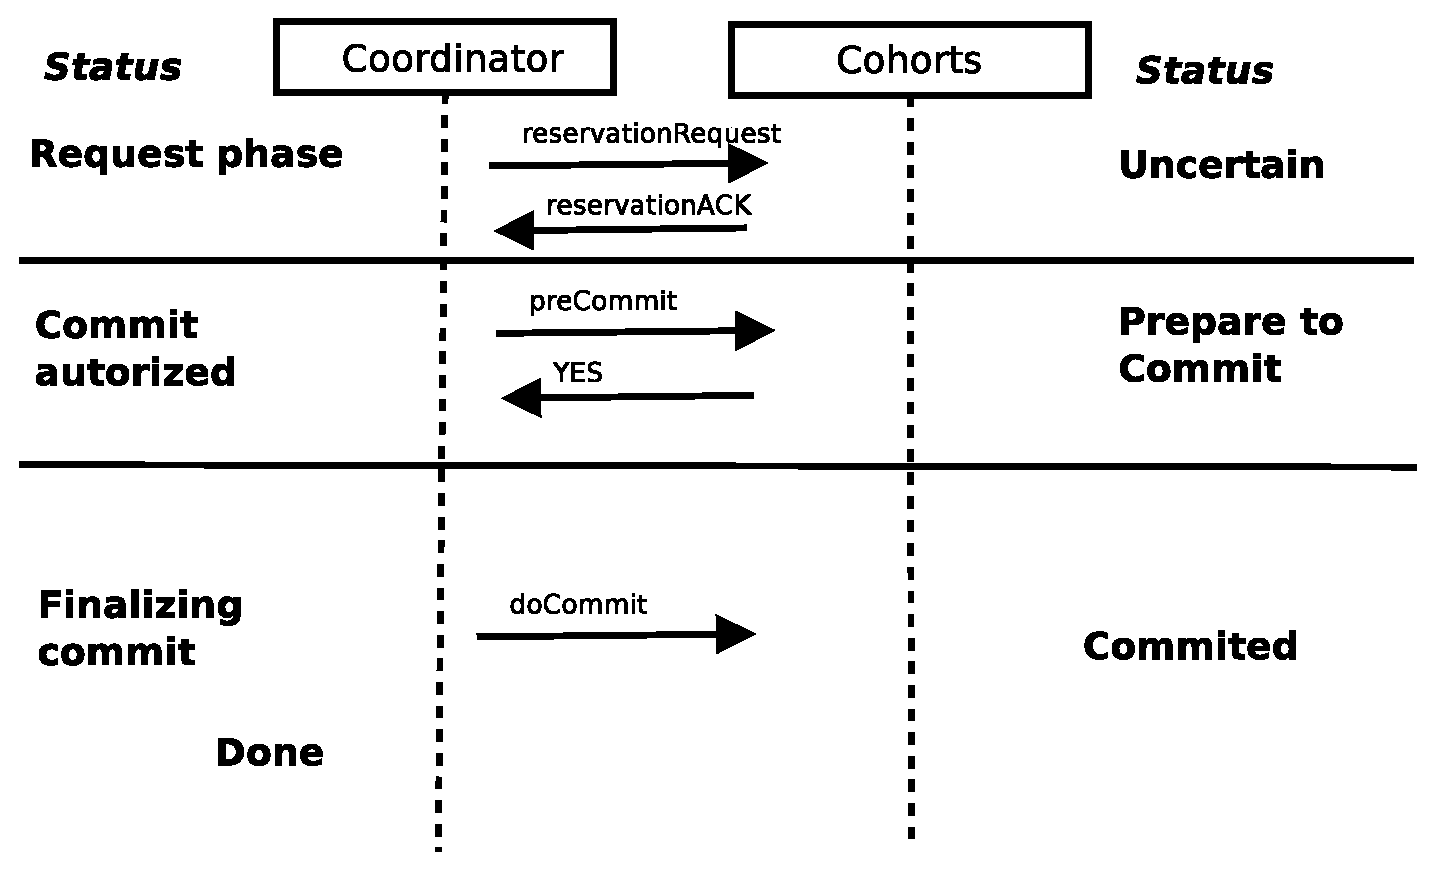
\includegraphics[scale=0.25]{3pcommit}
\end{lyxcode}
\caption{Client side 3 phase commit with modification for partition tolerance.}

\end{figure}

\begin{itemize}
\item Coordinator side (initiator of the event reservation):

\begin{enumerate}
\item The coordinator sends out reservation requests to all nodes. Nodes
then send their preferred list of slots (if any) to the coordinator
with RESERVATION-ACK messages, or decline the reservation request
with a RESERVATION-NACK message. If all nodes send RESERVATION-ACK
messages, the coordinator picks the first common slot agreed to by
the cohorts according to its preference and sends out a PRECOMMIT
message to all cohorts.
\item The coordinator then collects YES or ABORT messages from all the cohorts
depending on whether or not they agree to proceed further in the reservation.
\item If all nodes agree with a YES message, then the coordinator sends
all the cohorts a DOCOMMIT message, and it updates the reservation
status to COMMITTED, and the particular calendar slot to ASSIGNED.
This completes the reservation.
\item If at least one node sends an ABORT message, the coordinator aborts
the reservation, and sends out ABORT messages to all the cohorts,
causing them to abort as well.
\end{enumerate}
\item Cohort side (other participants in reservation):

\begin{enumerate}
\item The cohort receives a reservation request for a list of slots. If
it has at least one free slot from the list, then it responds with
those free slots in the form of a RESERVATION-ACK message. If none
of the requested slots are free, then the cohort responds with a RESERVATION-NACK.
\item If the cohort gets a PRECOMMIT message from a coordinator, then it
implies that all cohorts have responded for the reservation request
positively. The cohort then makes the following check:

\begin{enumerate}
\item If pre-commit-queue is empty, and there is no reservation under lock,
then lock this reservation and respond with a YES message.
\item If there is a reservation under lock, then add to the pre-commit-queue
if the reservation ID is newer than that under the lock. Do not respond
with any message at this point.
\item Else, if the reservation has an ID older than that in the lock, attempt
to abort newer reservation in favour of older one. This is done by
sending an ABORT message to the coordinator, and then waiting for
a response from the coordinator before performing the ABORT itself.
If the cohort receives a DOCOMMIT message after sending an ABORT,
it commits the currently locked reservation and aborts all reservations
in the queue.
\end{enumerate}
\item If the cohort receives a DOCOMMIT message, then commit the reservation
and change the respective slot's status to ASSIGNED.
\end{enumerate}
\end{itemize}
The procedure for aborting a reservation is as follows:
\begin{itemize}
\item Coordinator side: If the coordinator receives an ABORT message for
a particular reservation which has entered the precommit phase, then
it sends out ABORT messages to all cohorts. It then attempts to send
out PRECOMMIT messages for any other slots that all cohorts had previously
acknowledged for reservation. If there are no more slots left which
can be reserved, the coordinator declares the reservation to be ABORTED.
\item Cohort side: If the cohort decides to abort a reservation, it sends
an ABORT message to the coordinator. If it receives the ABORT message
back from the coordinator, it performs all the necessary cleanups
from the pre-commit queue, or the lock as is appropriate. If there
are no more potential slots available for the reservation to proceed,
then the reservation is marked as ABORTED.
\end{itemize}
Step 2.c protects against a potential deadlock situation which can
arise as follows:
\begin{enumerate}
\item Let there be a reservation R1 coordinated by node A, involving nodes
B and C. Let there also be a reservation R2, coordinated by D, which
has occured later than R1, involving nodes B and C as well.
\item One possible scenario that can arise is as follows: B has a lock on
reservation R1, and has R2 in its pre-commit queue. C has a lock on
reservation R2 and now receives the pre-commit message for R1. At
this point, note that reservation R2 cannot proceed since node B never
sent a YES message for R2, even though node C already has. But in
this event, node C sends out an ABORT message to its coordinator D,
causing it to abort reservation R2. Node C then promotes reservation
R1 from its pre-commit queue to its lock position, and responds with
a YES message to node A for reservation R1.
\item The older reservation R1 thus advances, and R2 is forced to abort.
\end{enumerate}

\subsection{Server Side: Leader Election and Replication}


\subsubsection{Leader Election}

All instances of a server knows about all other server instances.
Each instance has a unique id. The three servers regularly ping all other servers to determine, in a boolean fashion, its liveness. It is assumed that at most one server may fail at
any time. The first server alive will become the master. Servers are, in case of failure, rotated in a round-robin selection scheme. We assume that our failure detector is perfect, and that we're operating in a fail-stop model. Thus, it is not possible to determine if a server does not respond for a while due to heavy load. 

%Our leader election process is based on the Bully algorithm proposed
%by \cite{GarciaMolina}. In case of a server failure, when any other
%instance suspects that a server is unavailable, it will send a proposal
%to all other servers that X is unavailable. If all others agree, the
%server with the next highest ID is elected the new leader. The leader
%is selected in a round-robin fashion.

To handle network partitions, a server may only become a leader if
it is part of the cluster with a majority of the servers. Clients trying
to contact the minority cluster will not get any replies, and according
to a similar round-robin selection scheme of servers, eventually pick a server
from the majority cluster.


\subsubsection{Replication}

One of the design goals is to maintain a strong consistency among the replicas. Therefore, 
the master instance will propagate a write to at least one replica before
replying to the client. The propagation is synchronous
and utilises the broadcast component of the communication layer described
earlier. Thus, a server which receives a request will block until
it receives an acknowledgement from one correct replicas. The hit
this takes on performance can be justified by the fact that a replicated
set of servers which are highly available would most likely be on
a rack with a high bandwidth inter-connect. A replica is considered
alive as long as a recent heartbeat is available.

In case a replica, i.e an instance which is not the leader, gets a request from a client it will reply to the client informing it who is the actual master. The client will then be forced to resend its request to that server instance. This will increase the number of messages required, but keeps the design simpler. 

When a replica is started, in other words, when there already is at least one server alive, it will query this server with a replication request. The master will send its complete state - including the user table and its latest sequence number - to the replica. If a server crashes, a full synchronization is made. Servers maintain no persistent state on their own. Hence, the state is kept in memory.

%In case a replica, i.e an instance which is not the leader, gets an
%unexpected request from a client it will query the leader for the
%data, and retransmit the response to the client. Before propagating
%write requests to replicas, the leader maintains a log of all write
%records. When a server fails, and after a new leader is elected, the
%server instances will synchronize to ensure that the user lookup table
%and sequence number is aligned. Each write to the user lookup table
%updates a logical timestamp, such that ordering can be guaranteed.


\section{Evaluation}
\subsection{Results}

The following results were taken using 10 test cases provided at the project checkpoint. Each test case connects one or more clients to a set of servers. From test case 3 and onwards three servers are used. Test case 8 is unsupported as it requires migrating the coordination of a reservation to another user. Something not supported in our prototype. Moreover, the following measurements does not account for any messages sent by the servers. 

\begin{table}
    \begin{tabular}{|l|l|l|}
      \hline
      \multicolumn{3}{|c|}{Table 1: Test results} \\
      \hline
        \hline
        Test & Client 1 & Client 2 \\
        \hline
        1  & 2           & NA          \\ 
        2  & 2           & NA          \\ 
        3  & 2           & NA          \\ 
        4  & 2           & NA          \\ 
        5  & 8           & 5           \\ 
        6  & 8           & 6           \\ 
        7  & 17*          & 11          \\ 
        8  & Unsupported & Unsupported \\ 
        9  & 12          & 12          \\ 
        10 & 13          & 13          \\
        \hline
    \end{tabular}
\end{table}

Test case 1-4 only makes self-reservations with an increasing number of servers on-line, reaching a maximum of three. In test case 4, two slots are provided. However, as there are no previous slot reservations, and it is also self-reservation, no more than three messages will be used. 

In test case 5 two clients connect and Client 1 issues a reservation with Client 2 with one slot suggestion. Deducting the CONNECT and SEQUENCE\_NUMBER messages 6 messages are required for a successful multi-user reservation for the initiating client. For each message sent to another client a lookup message to determine the destination's uri is sent to the server. This causes the number of messages used for a reservation to double. In fact, only three messages are required for a successful reservation which does not pose any conflicts. Client 2 acks the first two messages in the reservation protocol: RESERVATION and PRECOMMIT. 

Test case 6 causes two clients two connect. Client 2 first initiates a self-reservation. Client 1 then tries to schedule a slot for the same slot that Client 2 just scheduled. As this slot is already confirmed, a new sequence will be initiated for the alternative slot. This reservation completes successfully. This causes the extra message from Client 2. 

In test case 7, the number of sent messages cannot be deterministically measured as it depends on how long the receiving client is disconnected from the system. Only when it comes back on-line is can the reservation successfully complete. 

Further, test case 7 was used to determine the average size of each message sent in the system. Still excluding server messages, counting 29 messages in total, the average size is 879 bytes with a standard deviation of 25 bytes. When accounting for server messages, which includes a substantial number of messages for its failure detector, the average size is 889 bytes, and a standard deviation of 30 bytes across a total of 231 messages. Message size was measured by serialising each message object into byte array and measuring its length. The larger deviation is due to the servers synchronization messages in which the user database is copied to the requesting server. 

Test case 9 and 10 includes more elaborate conflicts between the slots being reserved. However, all reservations eventually commit. Additionally, in test case 10 the master server is down for a period of time. This causes the client to search for a new master which results in one extra message. The system tolerates up to two server failures. If two fail simultaneously, each client may require up to two messages to determine the new master. 

\subsection{Analysis}
In this section we analyse our test results, suggest a few improvements, and briefly discuss our design choices for the software architecture. 

\subsubsection{Performance}
It is questionable why there are two messages being sent from the client in test case 1-4. At least one message in each test is the CONNECT message sent while the client is connecting to the server. For each reservation, irrespective of being a self-reservation or not, a sequence number is attached to it. One can argue that a self-reservation does not need a sequence number. That is left as an optimization. 

The messages are generally quite large. While measuring the size of an empty Message object, i.e without any attributes such as destination, source, type, or payload attached to it, it determined to be 853 bytes big. As we can see, the message overhead is not signficantly impacted by our message data but rather by .NET's method for binary serialization. Binary serialization is used over tcp channels in .NET remoting. Consequently, this tells us that optimising the content of the message would yield less improvements compared to focusing on minimising the total number of messages. For example, usernames to uri lookups are done one and one. As an improvement lookups could be batched together to reduce messages. 

Further, clients do not cache any lookups. Therefore a new lookup is performed for every send, even deffered sends. This explains the relatively high number of messages counted in test case 7 even though Client 2 only was down for a few seconds. Implementing a lookup cache for the clients was, however, not considered a primary task of this project. One would, in case a cache existed, have to consider for how long a cache entry is to be valid, and when it should be invalidated. 

There is one test case which is not supported at all, test case 8. This is because the coordinator is never online, at the same time, with all clients it is trying to reserve an event. Assuming that at one point in time, all clients have been on-line at the same time as the initiator, would solve this test case. If such an assumption is not made, the responsibility of completing a request has to be shared with all, or some, clients in the reservation. This could, for example, be done using a gossip mechanism: sharing the state of on-going reservations with the other clients that are online, such that they can complete it if a client which is down comes back online. 

\subsubsection{System Architecture}
One goal when designing the system was to minimize the number of remote entry points used between clients and between clients and servers. While Remote Procedure Calls offers developers the freedom to easily connect logic code with network code, it does comes with a price. Remote calls become interspersed with logic code and it becomes more difficult to follow the data and control flow. As the system required three components to be developed, the server, client and the puppet master, all of which required communication capabilities, we opted for an independent communication layer. The communication layer, used as is in all components, is fully decoupled from the services using it. In other words, the communication layer is completely unaware of what services are running on top. Instead each service registeres for the messages that it handles. Three important properties of this design choice are: 

\begin{enumerate}
\item The guarantees of the communication point to point links are centralised to one place in the system. Once implemented, it was available to all services and components. For example, resending messages to clients who have disconnected was added later in the development of the project and confined two only one place. 
\item It is easier to test and debug service and communication layer code independently. Communication bugs were all gathered in the same place as only one entry and exit point for messages exists in the system.
\item A separate channel for the puppet master was created using another instance of the communication layer. Ultimately giving the puppet master the same guarantees as the clients and the servers. 
\end{enumerate}  

Regarding server configuration, the design lacks a flexible way of easily adding more servers. This applies to client configuration as well as the replication service. A list of servers are provided in a configuration file to the client and the server. While that is ok, each component is hardcoded to only read maximum three servers, and will only rotate between these in case a server is disconnected. Improvments can be made by adding to the common library, a mechanism to read and manage the available servers. This limitation affects the scalability of the server component. 

Overall, the design choices made proved successfull. We were able to follow and use the architecture throughout the development and never resolved to any hacks which would be considered difficult or less elegant. 

\section{Conclusions\label{sec:Conclusions}}

In this paper, we have presented the design and architecture for RADICal,
a peer-2-peer distributed internet calendar service. The design is
made with testability in mind. The algorithms have been designed for
handling partition tolerance on the client side, and strong consistency
with availability on the server side.

\bibliographystyle{latex8}
\bibliography{latex8}

\end{document}
